\documentclass[11pt,letterpaper]{article}
\usepackage[T1]{fontenc}
\usepackage{lmodern}
\usepackage[margin=1in,headheight=15pt]{geometry}
\usepackage{amsmath,amssymb,bm,mathtools,microtype}
\usepackage{booktabs,tabularx,array,enumitem,needspace}
\usepackage{tikz,fancyhdr,xcolor,listings}
\usetikzlibrary{arrows.meta,calc}
\definecolor{linkblue}{RGB}{29,62,96}
\usepackage[colorlinks=true,linkcolor=linkblue,urlcolor=linkblue,citecolor=linkblue,menucolor=linkblue]{hyperref}
\usepackage[nameinlink,noabbrev]{cleveref}
\hypersetup{pdftitle={Fixed-Orientation Sliding Blocks: Contact Geometry, Guide Wrench and the CINDER Boundary},pdfauthor={CINDER technical note}}
\setlength{\parindent}{0pt}\setlength{\parskip}{.45em}
\setlength{\emergencystretch}{2em}
\clubpenalty=10000\widowpenalty=10000
\numberwithin{equation}{section}
\setlist{itemsep=.3em,topsep=.3em}
\pagestyle{fancy}\fancyhf{}
\fancyhead[L]{\small CINDER / Fixed-orientation sliding blocks}
\fancyhead[R]{\small CINDER 1.2.1}
\fancyfoot[L]{\small\Acrobatmenu{GoBack}{Previous view}}
\fancyfoot[C]{\thepage}\fancyfoot[R]{\small\hyperlink{contents}{Contents}}
\newcommand{\half}{\tfrac12}
\newcommand{\dd}{\mathrm d}
\newcommand{\er}{\bm e_r}\newcommand{\et}{\bm e_t}\newcommand{\ez}{\bm e_z}
\newcolumntype{Y}{>{\raggedright\arraybackslash}X}
\lstset{basicstyle=\small\ttfamily,breaklines=true,columns=fullflexible,frame=single}
\begin{document}
\begin{center}
{\small CINDER TECHNICAL NOTE / OCTOBER 17, 2026}\par\vspace{.7em}
{\LARGE\bfseries Fixed-Orientation Sliding Blocks}\par\vspace{.4em}
{\large Contact Geometry, Guide Wrench, and the Common Boundary}
\end{center}

A sliding centrifugal weight can move outward while two surfaces determine its
axial position. The fixed cup carries one surface; the movable sheave carries
the other. Once a guide prevents relative rotation of the weight, those two
contact constraints can determine its translation from sheave closure alone.
The resulting motion supplies the same effective mass and shaft inertia as
any other mechanism admitted by the common boundary \cite{common}.

That reduction does not make the block torque-free. Contact forces generally
have different moment arms about its centre of mass (COM), and the block still
rotates in space with the shaft. This note derives the contact motion first,
then the inertia functions, complete ideal-guide demand, and the impulses
needed to retain the contacts at a velocity reset.

The supported model is a CVTech-style sliding-block arrangement. The examples
are synthetic profiles, not measured CVTech hardware. A particular cup, weight,
insert, moving sheave, and anti-rocking guide still require their actual
geometry and mass properties before this model can represent that assembly.

\hypertarget{contents}{}\setcounter{tocdepth}{1}\tableofcontents
\clearpage
\section{Attachments, coordinates, and retained motion}

Use the right-handed local basis $(\er,\et,\ez)$, with $\ez$ along the shaft
and $\et=\ez\times\er$. The local sheave coordinate $x$ is positive in closure;
the moving contact track translates by $+x\ez$. The lower track is axially
fixed in the shaft frame. Both tracks and the orientation guide co-rotate
with the shaft at angular speed $\omega$ and acceleration $\alpha$.
The origin of $x$ is arbitrary: positive denotes its direction, not a
restriction $x\geq0$. In particular, CINDER's secondary opens into negative
local coordinates during upshift. The supplied profiles and compiled interval
must cover that signed travel.

Let $(R(x),Z(x))$ locate a datum fixed in the block. The block does not rotate
relative to these local axes. Its COM offset from the datum is the fixed
vector $(c_r,c_t,c_z)$, so the COM coordinates are
\begin{equation}
 r=R+c_r,\qquad y=c_t,\qquad z=Z+c_z.
\end{equation}
Separating this datum from the COM is essential for tuning inserts: changing
an insert can move the COM without moving either contacting face.

The complete identical set has mass $M$ and contains $n$ blocks. One block has
mass $M/n$. Store the centroidal inertia tensor per unit mass as $\bm K$,
expressed in $(r,t,z)$ axes. Thus $\bm I_{C,\mathrm{set}}=M\bm K$ is the sum of
corresponding local centroidal tensors, and $\bm I_{C,1}=M\bm K/n$ belongs to
one block. Off-diagonal entries are the entries of the inertia tensor itself:
for example, $K_{rz}=-\int u_r u_z\,\dd m/m$. They are not unsigned geometric
products of inertia.

The mass set is constant. The cup and rigid sheave masses remain in the host
pulley accounting; they are not included in $M$. Springs and belt loads are
separate elements. The contacts here are frictionless and unilateral. The
initial guide is an explicit ideal constraint: it supplies a tangential force
through the COM and an arbitrary holding couple, with no frictional loss.
Physical guide capacities are unknown, rather than inferred from the outline.

\section{Two finite profiles determine the body translation}
\label{sec:contacts}

Each contact face is a finite graph in a meridional section. Write the lower
and upper block faces as $z=b_\ell(u)$ and $z=b_u(u)$, where $u$ is radial
position relative to the body datum. The two faces share a declared interval
$[u_a,u_b]$, and $b_u>b_\ell$ throughout it. The fixed and moving tracks are
$z=f_\ell(\rho)$ and $z=f_u(\rho)+x$, respectively, on finite radial domains.
The whole block footprint must remain within both modelled track domains.

At a trial datum pose $(R,Z)$, define the signed axial gaps
\begin{align}
 g_\ell(u;R,Z)&=Z+b_\ell(u)-f_\ell(R+u),\\
 g_u(u;R,Z,x)&=f_u(R+u)+x-Z-b_u(u).
\end{align}
A nonnegative gap means separation without penetration. A retained contact
requires the minimum gap on that face to be zero. This compares the full
finite face, rather than selecting a tangent while ignoring another part of
the same face that might penetrate the track.

The contact equations above do not prescribe a circular cup or a particular
block outline. CINDER 1.2.1 accepts user-defined twice continuously
differentiable piecewise polynomial graphs, alongside exact lines, quadratics
and circular-arc graphs. On a radial interval $[a_j,a_{j+1}]$, a polynomial
profile is stored as
\begin{equation}
 f(\rho)=f_0+\sum_{k=0}^{d_j}c_{jk}t^k,
 \qquad t=\frac{\rho-a_j}{a_{j+1}-a_j}.
 \label{eq:profile-polynomial}
\end{equation}
The coefficients are axial lengths. Normalizing the independent coordinate
avoids powers of very small metre-valued intervals in the root calculation.
Seams agree through the second derivative. Point input explicitly interpolates
a cubic spline, or a quintic when requested; it does not silently fit or smooth
measurement noise. Curves and their actual derivatives, rather than a display
mesh, determine contact.

These remain meridional graphs. Overhangs, independent rocking and
three-dimensional saddle contact require a different contact construction.
That is a scope of this translation provider, not a restriction of the common
material-motion boundary. The block's full mass distribution remains separate
from its selected contacting faces.

\subsection{Finding the whole contact set}

The minimum gap can occur at an endpoint, at a profile seam, at any stationary
point, or throughout a constant-gap interval. The implementation enumerates
all of these candidates over the finite face. For polynomial pieces, the gap
is polynomial and its derivative roots supply all interior candidates,
including repeated stationary roots. Derivative roots partition the normalized
interval into monotone pieces for bracketed root isolation. Curvature may
change sign and there may be several local minima; neither condition is a
reason to select only one guessed tangent.

With a circular graph, stationarity involves a square root. Squaring produces
a polynomial candidate equation. Every candidate is then checked against the
original unsquared slope equation to remove extraneous roots. The opposite
branches of a circle are not mistaken for a constant gap merely because their
squared derivative expressions agree. These constructions are evaluated in
floating-point arithmetic with declared numerical resolutions.

Retain all candidates attaining the minimum to that resolution. A pair
$(u,u)$ denotes a point and $[a,b]$ a complete flat contact interval. The
representative coordinate used to draw a normal is not a pressure centroid.
This distinction will matter for the guide moment even when the clamping
resultant is determined.

\subsection{Establishing a regular configuration branch}

To reduce the two equations, put
\begin{equation}
 A(R)=\max_u[f_\ell(R+u)-b_\ell(u)],\qquad
 C(R)=\min_u[f_u(R+u)-b_u(u)].
\end{equation}
The lower contact gives $Z=A(R)$ and the upper contact gives
\begin{equation}
 x=A(R)-C(R).
 \label{eq:inverse}
\end{equation}
Disjoint bounds on the slopes of the active tracks establish that the
derivative of this function is nonzero. A bracketed scalar solve then gives
the unique $R$ within the declared radial window. Track-wide bounds are tried
first. If they overlap, a contact enclosure excludes regions of the face
which cannot attain the minimum gap, and the radial window is subdivided.
To see the exclusion, let a trial face point give a uniform upper bound on
the minimum gap over a radial interval. Any face subinterval whose lower gap
bound exceeds it cannot contain contact. Profile extrema bound both values
and derivatives throughout each interval.

Monotone closure alone does not establish smooth motion: the identity of the
minimum can switch between separated parts of a curved track. On the reachable
radial path, additional local bounds establish an isolated regular minimum or
a retained endpoint. Affine tracks admit an important further case: the gap
separates into a function of $u$ and an affine function of $R$. Its minimizing
contact set is fixed even if it contains several points or a whole face, so
its envelope remains smooth. \Cref{sec:distributed} treats the associated loads.

A numerical enclosure failure is not proof that the proposed hardware is
impossible. The implementation reports the unresolved interval and contact.
It does not hide a transition by blending two motion curves. Changes of
contact-set cardinality currently require separate branch handling. The
bounds use floating-point stationary-root calculations; the subsequent
interpolation diagnostics are separate sampled checks.

Endpoint contact is allowed only when explicitly requested. It is an ideal
point contact at a finite face endpoint with the smooth track's normal.
A rounded nose of finite radius must be represented by its actual geometry
if its change to the contact path matters. Neither an unknown corner radius
nor a pressure centroid is fitted automatically.

\section{Motion ratios from the same contact constraints}

Let $u_\ell$ and $u_u$ be the active face coordinates and let
$s_i=f_i'(R+u_i)$ be the corresponding track slopes. At an interior tangent,
$b_i'(u_i)=f_i'(R+u_i)$. The derivative of the minimum gap with respect to its
minimizer vanishes; at a retained endpoint, $u_i$ is constant. In either case,
differentiating the two closed gaps gives
\begin{equation}
 Z'=s_\ell R',\qquad Z'=1+s_u R'.
\end{equation}
Consequently,
\begin{equation}
 D=s_\ell-s_u,\qquad R'=\frac1D,\qquad Z'=\frac{s_\ell}{D}.
 \label{eq:first}
\end{equation}
The constraint Jacobian has rows $(-s_\ell,1)$ and $(s_u,-1)$.
As $D$ approaches zero the geometry ceases to determine a regular translation.
The implementation bounds its condition number over the branch and rejects
ill-conditioned windows rather than clipping the motion ratio.

Curvature changes the active track slope as the block moves. At an interior
contact, differentiation of the tangency condition with respect to $R$ yields
\begin{equation}
 u_{i,R}=\frac{f_i''}{b_i''-f_i''},\qquad
 s_{i,R}=f_i''(1+u_{i,R}).
 \label{eq:contact-migration}
\end{equation}
At a retained endpoint $u_{i,R}=0$. All profile derivatives in this expression
are evaluated at the active material coordinates. Thus the second motion
ratios are
\begin{equation}
 R''=-(s_{\ell,R}-s_{u,R})(R')^3,\qquad
 Z''=s_\ell R''+s_{\ell,R}(R')^2.
 \label{eq:second}
\end{equation}
The fixed COM offset does not affect these derivatives: $r'=R'$, $z'=Z'$,
and likewise for second derivatives.

\subsection{Mass geometry is independent of contact selection}

The contact faces determine compatible motion; the retained material determines
mass, COM and inertia. A uniform extruded polygon can be reduced using its area
moments. A smooth body bounded by two profiles can instead be integrated
directly, without using the tessellated drawing. Both constructions return
the COM and full centroidal tensor per unit mass in the body datum; the
supplied total group mass fixes the uniform density. Inserts or nonuniform
material require their actual moments. Additional cup or sheave backing is
CVT material and never enters this weight-mass reduction.

\section{Mass motion supplies the four quantities}
\label{sec:inertia}

Because orientation is fixed relative to the shaft frame, every material point
has the same relative translation velocity $(r',0,z')\dot x$. Its spin about
the COM still contributes to shaft-rotation energy. Integrating the material
velocity therefore gives
\begin{equation}
 T_f=\half M\bigl[(r')^2+(z')^2\bigr]\dot x^2
       -M c_t r'\omega\dot x
       +\half\bigl[M(r^2+c_t^2)+M K_{zz}\bigr]\omega^2.
\end{equation}
The mixed coefficient is $B_f=-M c_t r'$. Fixed orientation alone does not
remove it. The initial implementation requires $c_t=0$; it does not infer
cancellation from equally spaced blocks. With that condition established,
\begin{equation}
\boxed{\begin{aligned}
 M_f&=M[(r')^2+(z')^2],&
 M_f'&=2M(r'r''+z'z''),\\
 J_f&=Mr^2+M K_{zz},& J_f'&=2Mrr'.
\end{aligned}}
\label{eq:maps}
\end{equation}
These are total-set quantities. The count $n$ does not multiply them again.
The tensor must be finite and symmetric, with nonnegative principal inertias
satisfying the triangle inequalities. These checks establish a possible
inertia tensor; they do not establish that supplied mass properties actually
belong to the specified outline and inserts.

The common CINDER element \cite{common} consumes \cref{eq:maps} and supplies
\begin{equation}
 F_x=\half J_f'\omega^2-M_f\ddot x-\half M_f'\dot x^2,
 \qquad \tau=-J_f\alpha-J_f'\dot x\omega.
 \label{eq:loads}
\end{equation}
There is one implementation of these relations in
\texttt{CentrifugalInertiaForce}. The sliding-block provider adds the geometry
and contact policy; it does not carry another transient force law. The same
$M_f$ and $J_f$ enter kinetic energy and event projection.

\section{Contact reactions and the torque on each block}
\label{sec:wrench}

The four maps describe work and kinetic energy, but their reduction has
eliminated the individual constraint reactions. Recover those reactions from
the block's free body before deciding whether the contact branch is admissible.
The contact normals on the block, written as radial--axial pairs, are
\begin{equation}
 \bm n_\ell=\frac{(-s_\ell,1)}{\sqrt{1+s_\ell^2}},\qquad
 \bm n_u=\frac{(s_u,-1)}{\sqrt{1+s_u^2}}.
\end{equation}
With compression positive, the total corresponding normals satisfy
\begin{equation}
 [\bm n_\ell\ \bm n_u]
 \begin{bmatrix}N_\ell\\N_u\end{bmatrix}
 =M\begin{bmatrix}
 r'\ddot x+r''\dot x^2-r\omega^2\\
 z'\ddot x+z''\dot x^2
 \end{bmatrix}.
 \label{eq:normals}
\end{equation}
The tangential acceleration is separate. The ideal guide supplies
\begin{equation}
 G_t=M(r\alpha+2\omega r'\dot x).
 \label{eq:guide-force}
\end{equation}
The $2\omega r'\dot x$ term is the tangential acceleration associated with
radial motion in the rotating frame. Neither contact normal in this model has
a tangential component.

The guide must also prevent relative rocking. Let $\bm a_i$ run from the COM
to contact $i$, let $\bm N_i=N_i(n_{i,r},0,n_{i,z})$, and use the full
centroidal tensor. The required holding couple is
\begin{equation}
 \boxed{\bm G_C=M\bm K\,(\alpha\ez)
       +(\omega\ez)\times[M\bm K(\omega\ez)]
       -\sum_{i=\ell,u}\bm a_i\times\bm N_i.}
 \label{eq:guide-moment}
\end{equation}
The spin terms have components
\begin{equation}
 M\bigl(K_{rz}\alpha-K_{tz}\omega^2,\quad
        K_{tz}\alpha+K_{rz}\omega^2,\quad K_{zz}\alpha\bigr).
\end{equation}
Even at constant shaft speed, a nonzero product of inertia can require a
transverse couple. Even with zero products, the two contact moments need not
cancel. A single shaft-axis gyration radius cannot determine this full demand.

For the straight synthetic case at $x=7.5\,\mathrm{mm}$,
$r=57\,\mathrm{mm}$, $M=0.75\,\mathrm{kg}$ and
$\omega=350\,\mathrm{rad\,s^{-1}}$, steady contact gives
$F_x=2094.75\,\mathrm N$. The contact-only holding couple has magnitude
$51.0595\,\mathrm{N\,m}$ in corresponding local axes, or
$17.0198\,\mathrm{N\,m}$ per block for $n=3$.
\Cref{fig:fbd} shows why the lines of action do not remove this moment.

\begin{figure}[htbp]\centering
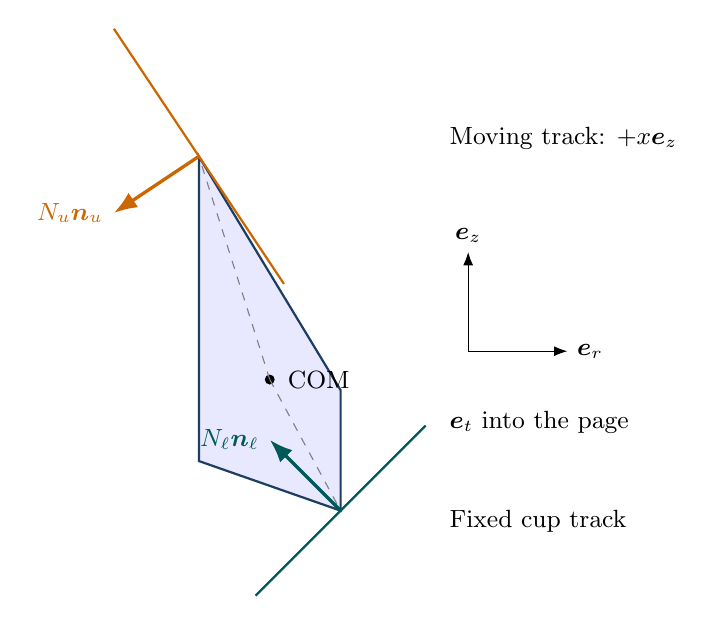
\begin{tikzpicture}[x=.18cm,y=.18cm,>=Latex,font=\small]
 \filldraw[fill=blue!9,draw=linkblue,thick] (-5,-5.75)--(5,-9.25)--(5,-.75)--(-5,15.75)--cycle;
 \draw[teal!70!black,thick] (-1,-15.25)--(11,-3.25);
 \draw[orange!80!black,thick] (-11,24.75)--(1,6.75);
 \fill (0,0) circle (.35) node[right=3pt]{COM};
 \draw[gray,dashed] (0,0)--(5,-9.25);
 \draw[gray,dashed] (0,0)--(-5,15.75);
 \draw[->,teal!70!black,very thick] (5,-9.25)--(0,-4.25) node[left]{$N_\ell\bm n_\ell$};
 \draw[->,orange!80!black,very thick] (-5,15.75)--(-11,11.75) node[left]{$N_u\bm n_u$};
 \node[anchor=west] at (12,17){Moving track: $+x\ez$};
 \node[anchor=west] at (12,-10){Fixed cup track};
 \draw[->] (14,2)--(21,2) node[right]{$\er$};
 \draw[->] (14,2)--(14,9) node[above]{$\ez$};
 \node[anchor=west] at (12,-3){$\et$ into the page};
\end{tikzpicture}
\caption{Local section of the straight synthetic block at the stated pose.
The contact arms are measured from the COM. Shaft-induced centripetal
acceleration is supplied by the resultant radial force; the guide couple must
balance the contact moment as well as any centroidal spin demand. The track
segments indicate contact surfaces, not complete cup or sheave solids.}
\label{fig:fbd}
\end{figure}

All normals and guide components above are sums of corresponding local values;
divide by $n$ for one pocket. They are not a global transverse-vector sum around
the pulley. Symmetric cancellation at assembly level does not unload each
pocket. Circumferential sidewall forces alone also cannot resist a moment
about the tangential axis: an anti-rocking feature must constrain that motion.
A specified real guide may transmit radial and axial forces too, in which case
\cref{eq:normals} must be replaced by the complete guide/contact equilibrium.

For the present ideal guide, the moving track delivers
$F_x=-N_u n_{u,z}$. This agrees with \cref{eq:loads} for the exact constraint
motion. The runtime contact policy uses both $N_\ell$ and $N_u$ at the actual
solved accelerations. It rejects resolved tension. Raw reactions remain
available; a numerical-resolution check described below distinguishes
unresolved near-zero values from a required tensile contact.

\section{Clamping with an undetermined pressure location}
\label{sec:distributed}

Two matching flat faces need not determine a single pressure application point.
Nevertheless, the flat moving track has one normal direction and supplies one
closed-gap equation. For $b_u(u)=b_0+s_u u$ and
$f_u(R+u)=f_0+s_u(R+u)$, that equation is
\begin{equation}
 Z=f_0-b_0+s_uR+x.
\end{equation}
The coordinate $u$ has cancelled. Combined with the fixed-cup envelope
$Z=A(R)$, it can determine a unique regular translation. Its derivatives and
the four inertia quantities follow as before. The two common normal directions
then determine the total forces in \cref{eq:normals}. Thus unknown pressure
location does not, by itself, make clamping undetermined.

A nonconvex block may likewise touch an affine track at two separated points.
Both normals have the same direction, and their nonnegative pressures add to
one force resultant. The pressure centroid can lie in the convex hull of the
contact set, even if the material between the two points is not in contact.
The API retains the actual separate points instead of drawing this convex
hull as a physical contact patch.

The remaining ambiguity concerns moment. Let $\mathcal U_i$ be the contact set
on face $i$ and put
\begin{equation}
 \bm q_i(u)=-\bm a_i(u)\times[N_i\bm n_i],\qquad
 \bm G_0=M\bm K(\alpha\ez)
   +(\omega\ez)\times[M\bm K(\omega\ez)].
\end{equation}
For each component $k$, the ideal-guide demand is bounded by
\begin{equation}
 G_{0,k}+\sum_i\min_{u\in\mathcal U_i}q_{i,k}(u)
 \ \leq G_{C,k}\leq\
 G_{0,k}+\sum_i\max_{u\in\mathcal U_i}q_{i,k}(u).
 \label{eq:guide-bounds}
\end{equation}
For the admitted common-normal meridional contacts, only the tangential
component has pressure-location uncertainty. On a flat interval its moment
is affine in $u$, so the endpoints determine its extrema; isolated contact
points are evaluated individually. These bounds include the full centroidal
spin demand. A unique contact point gives coincident bounds and recovers
\cref{eq:guide-moment}. When these bounds differ, the single guide moment is marked undetermined.
Coincident bounds still give a unique moment, including the unloaded case. The same construction applies to
impulses using $P_i$ and the centroidal angular-momentum jump.

As a closed-form check, take a fixed affine cup of slope $0.8$, a matching
moving face of slope $-0.5$, and a lower block face
\begin{equation}
 b_\ell(u)=0.8u+c(u^2-a^2)^2,
 \quad a=0.004\,\mathrm m,\quad c=10^6\,\mathrm{m^{-3}}.
\end{equation}
The lower face contacts at the two distinct points $u=\pm a$.
With the open datum $R_0=0.05\,\mathrm m$, $Z_0=0$, and suitable upper-face
thickness, the two gap constraints give
\begin{equation}
 R=R_0+\frac{x}{1.3},\qquad Z=\frac{0.8x}{1.3}.
\end{equation}
For zero COM offset and held closure, the mechanism's closing contribution is
$F_x=Mr\omega^2/1.3$. Springs and belt loads enter the host balance separately. It is unique although the guide moment has a finite
pressure-dependent range. This example tests multiple global minima and flat
face contact without using the compiled motion as its expected solution.

\section{Retaining the contacts through a velocity reset}
\label{sec:impact}

An instantaneous reset changes velocities at one fixed configuration. Smooth
centrifugal, Coriolis, spring, and applied-torque terms do not supply finite
impulses over that zero-duration interval. If the same two contacts and guide
remain active, their required impulses follow from the velocity jumps:
\begin{align}
 [\bm n_\ell\ \bm n_u]
 \begin{bmatrix}P_\ell\\P_u\end{bmatrix}
   &=M\begin{bmatrix}r'\\z'\end{bmatrix}\Delta\dot x,\\
 P_t&=Mr\Delta\omega,\\
 \bm L_C&=M\bm K(\Delta\omega\ez)
             -\sum_i\bm a_i\times\bm P_i.
 \label{eq:impulse}
\end{align}
The normal impulses must be compressive. The ideal guide is permitted to carry
its computed force impulse and couple impulse, but its real capacity is still
unknown. A positive running normal force does not establish the sign of these
impulses.

For the straight case, arresting $\dot x=+0.1\,\mathrm{m\,s^{-1}}$ with no
shaft-speed jump requires
\begin{equation}
 (P_\ell,P_u)=(-0.00848528,\ 0.04326662)\,\mathrm{N\,s}.
\end{equation}
The lower contact would have to pull. The stop therefore cannot retain this
branch, despite admissible pre-impact running forces. CINDER exposes the
normal-impulse margins on candidate projections and rejects an inadmissible
selected transition. Resolving what happens after release needs a different
contact topology or an additional dynamic coordinate; this version does not
invent that motion.

\section{Compilation, inputs, and limits in CINDER 1.2.1}

\texttt{SlidingBlockGeometry} stores the four profiles, radial branch window,
local axial interval, and explicit endpoint-contact policy.
\texttt{SlidingBlockMass} stores total mass, count, COM offset, and the full
centroidal tensor per mass. \texttt{SlidingBlockSpec} combines these with the
required \texttt{ideal\_fixed\_orientation} guide declaration.
The saved component kind is \texttt{sliding\_block\_flyweight}. Distances are
metres, mass is kilograms, profile curvature is inverse metres, and tensor
entries are square metres. The JSON examples in the package example folder provide complete component
records, including a noncircular cup and a nonconvex multi-contact weight;
they are not full CVT assemblies.

The compiler solves geometry outside the runtime RHS and constructs a common
$C^2$ piecewise quintic Hermite representation of $R,Z$ and cached paths for
the contact-set endpoints. Values and the first two body-motion derivatives
come from the same contact construction. Contact coordinates need accurate
values; their second derivatives need not agree across a $C^2$ profile seam. Both inertia
functions and their derivatives use this one compiled motion. Contact
locations and normals also use the cached representation; no root solve is
performed inside the closure iteration.

Starting from eight intervals, the compiler tests three interior points per
cell and subdivides failed cells. Position errors include the contact-set
endpoints; derivative errors concern $R,Z$. Its absolute tolerances are
$2\times10^{-10}\,\mathrm m$ for positions,
$2\times10^{-7}$ for first derivatives, and
$2\times10^{-4}\,\mathrm{m^{-1}}$ for second derivatives.
The compilation report records the largest observed errors. These are sampled
interpolation diagnostics, distinct from the interval tests establishing the
contact branch; they are not rigorous continuum bounds on interpolation error.
The cache is keyed by the immutable geometry, so mass changes reuse the motion.
Queries outside the compiled axial interval raise an error without extrapolation.

One sliding-block element represents the entire distributed group on a pulley.
Python construction and saved-document validation reject duplicate groups;
change the total mass instead. If an insert also changes the distribution,
update the COM and tensor rather than scaling mass alone.

\subsection{Numerical resolution at zero contact load}

A mathematically zero reaction can evaluate slightly below zero when large
inertial terms cancel. There is also a small tangency discrepancy because the
motion derivatives and profile normals are evaluated from a finite interpolant.
Neither effect calls for a fixed allowance in newtons. Measure the discrepancy
at the actual pose instead.

Let $H=[\bm n_\ell\ \bm n_u]$ and $\bm v_x=(r',z')^T$. Exact closed-contact
motion gives $\bm v_x^T\bm n_\ell=0$ and
$\bm v_x^T\bm n_u=n_{u,z}$: the fixed track does no work and the moving
track translates with unit axial speed per unit $\dot x$. Define the two
computed residuals by
\begin{equation}
 (d_\ell,d_u)=\bm v_x^T H-(0,n_{u,z}),\qquad
 E=|d_\ell N_\ell|+|d_u N_u|.
 \label{eq:work-residual}
\end{equation}
Projecting \cref{eq:normals} onto $\bm v_x$ shows that
$|F_x+N_u n_{u,z}|\leq E$, where $F_x$ is the common boundary's force
from \cref{eq:loads}. Projection onto $\bm v_x-(0,1)^T$ gives the
corresponding fixed-track identity. Thus $E/|n_{i,z}|$ measures each recovered
normal's discrepancy from its scalar virtual-work identity.

For arithmetic resolution, split the right side of \cref{eq:normals} into
its acceleration, curvature and centrifugal vectors $\bm b_k$ and set
\begin{equation}
 S_i=\left[|H^{-1}|\sum_k|\bm b_k|\right]_i,\qquad
 \eta_i=\frac{E}{|n_{i,z}|}
       +4096\,\epsilon\max(N_0,S_i).
 \label{eq:normal-resolution}
\end{equation}
Absolute values of vectors and matrices are componentwise. Here $\epsilon$
is machine precision and $N_0=1\,\mathrm N$ is the reference scale in CINDER's
existing roundoff convention. The inverse matrix accounts for amplification
by the contact directions. Only the reported admissibility margin is snapped
to zero when $|N_i|\leq\eta_i$; the raw reaction, guide wrench and common
force law are unchanged. A normal below $-\eta_i$ is rejected.

The same calculation applies to \cref{sec:impact}, using its momentum-jump
vector in place of $\sum_k\bm b_k$, normal impulses in
\cref{eq:work-residual}, and a $1\,\mathrm{N\,s}$ reference scale.
These checks quantify local numerical consistency. They neither certify
hardware capacity nor replace the compiler's separate interpolation diagnostics.

\begin{center}\begin{tabularx}{\textwidth}{@{}p{.25\textwidth}Y@{}}
\toprule
Limit & Implemented response\\\midrule
Invalid inputs & Reject non-finite values, impossible tensors, nonpositive thickness,
invalid domains/count, and a nonzero tangential COM offset.\\[.4em]
Geometric branch & Search all finite-face minima. Establish regular reachable
motion; report unresolved enclosures, contact-set transitions, insufficient
support and ill-conditioned kinematics separately. Flat common-normal contact
sets retain clamping and guide-moment bounds.\\[.4em]
Operating state & Evaluate both normal forces with the solved local acceleration;
reject contact loss. Report the complete ideal-guide demand separately.\\[.4em]
Velocity reset & Resolve both normal impulses and reject a selected reset requiring
tension. Direct projection callers must check the returned margins.\\[.4em]
Hardware envelope & Speed, stress, pressure, real guide capacity, supporting-solid
clearance, and three-dimensional interference require additional supplied data
and checks; no universal safe RPM is derived from these profiles.\\\bottomrule
\end{tabularx}\end{center}

The mechanism may mount on either pulley when both contact tracks co-rotate
with its shaft. A relative sheave helix is rejected. The host retains the full
local-to-shared acceleration relation and the separate sheave/cup mass
ownership. Point/segment authoring and the frontend preview service remain a separate
application change; no template cup radius, backing thickness or arbitrary
sample dimension bound is introduced by this core contact representation. The research viewer now imports CINDER's Python
mechanics and contracts exported response coefficients in JavaScript; it does
not maintain another contact-force equation.

\section{Verification and what it establishes}

The straight case recovers the force form used in Messick's straight-ramp
model \cite{messick}: $M_f'=0$ and the steady closing force is $Mr r'\omega^2$,
with total $M$ replacing a per-weight mass times count. This tests the force
scale and geometry convention, not the dimensions of a particular machine.

The core smoke tests also differentiate inertial Cartesian trajectories of
eight material masses. Only direct geometric positions are reused; the
expected force, shaft torque and kinetic energy do not use the four-map
formula. Three profile families, forward/reverse/zero shaft rotation, and both
host shaft channels are exercised. Other checks cover derivative consistency,
COM changes at fixed geometry, opposite products of inertia at identical four
maps, saved-document/schema round trips, named running contacts, and valid and
invalid stop projections. A short coupled neutral-shift transient checks
primary angular-momentum conservation while axial motion changes shaft inertia.

The existing fixed-pivot launch regression remains a separate check of the
common-boundary migration. None of these checks measures real CVTech guide
capacity, contact pressure, wear, or post-release motion. Their practical
conclusion is that the stated constrained model supplies consistent continuous
and impulsive mechanics and explicitly identifies conditions it cannot retain.

\appendix
\section{Contact-coordinate derivatives for the interpolant}

The compiler also needs derivatives of the material contact coordinate. With
$h=u_R=f''/(b''-f'')$ at an interior tangent, another differentiation gives
\begin{equation}
 u_{RR}=\frac{f'''(1+h)^2-b'''h^2}{b''-f''},\qquad
 u'=hR',\qquad u''=hR''+u_{RR}(R')^2.
\end{equation}
All of these derivatives are zero for a retained material endpoint. Lines and
quadratics have zero third derivative. For the circle used in
\cref{sec:contacts}, with $d=\rho-\rho_0$,
\begin{equation}
 f''=\frac{\sigma a^2}{(a^2-d^2)^{3/2}},\qquad
 f'''=\frac{3\sigma a^2d}{(a^2-d^2)^{5/2}}.
\end{equation}
The open-semicircle domain and branch checks keep these values finite. A
contact-mode change requires a separate branch; this derivative construction
does not assign a smoothed corner motion.

\begin{thebibliography}{9}
\bibitem{common} \emph{General Centrifugal Mechanisms: From Compatible Motion to
Clamping Force and Shaft Coupling}. Revision 4; canonical CINDER 1.2.1 edition.
\href{../common_boundary/formulation.pdf}{Common-boundary document}.
\bibitem{fixed} \emph{Clamping Mechanism Implementations: The Fixed-Pivot Roller
Flyweight}. CINDER 1.2.0 edition.
\href{../fixed_pivot/formulation.pdf}{Fixed-pivot document}.
\bibitem{manuscript} Kai Arseneau and W. Spencer Smith.
\emph{A First-Principles Dynamic Model of a Rubber V-Belt CVT for General
Transient Simulation: With Mechanical Actuation and Traction-Limited Torque
Transfer}. Supplied manuscript, October 1, 2026; Sections 3.2, 3.3 and 3.6.
\bibitem{messick} M. J. Messick. Supplied 2018 thesis, Section 9.4.1,
printed page 109 (PDF page 118), Eq. 9.2. Used for the straight-ramp force limit;
the dimensions in this note are synthetic.
\end{thebibliography}
\end{document}
